\documentclass{beamer}
\usepackage{ctex, hyperref}
\usepackage{subfigure}
\usepackage[T1]{fontenc}
\usepackage[backend=bibtex,bibstyle=gb7714-2015,citestyle=gb7714-2015]{biblatex}
\setlength{\bibitemsep}{3bp}
\renewcommand*{\bibfont}{\zihao{5}\linespread{1.27}\selectfont}
\addbibresource{ref.bib}
\usefonttheme[onlymath]{serif}
% other packages
\usepackage{latexsym,amsmath,xcolor,multicol,booktabs,calligra}
\usepackage{graphicx,pstricks,listings,stackengine}

\author{吴熙楠}
\title{$Quantum\quad Hall\quad Effect$}
\subtitle{$Shubnikov-de\quad Haas\quad Oscillation$}
\institute{北京大学物理学院}
\date{\today}
\usepackage{PKU}
\logo{
\includegraphics[scale=0.04]{pic/PKU_logo.png}}
% defs
\def\cmd#1{\texttt{\color{red}\footnotesize $\backslash$#1}}
\def\env#1{\texttt{\color{blue}\footnotesize #1}}
\definecolor{deepblue}{rgb}{0,0,0.5}
\definecolor{deepred}{rgb}{0.6,0,0}
\definecolor{deepgreen}{rgb}{0,0.5,0}
\definecolor{halfgray}{gray}{0.55}

\lstset{
    basicstyle=\ttfamily\small,
    keywordstyle=\bfseries\color{deepblue},
    emphstyle=\ttfamily\color{deepred},    % Custom highlighting style
    stringstyle=\color{deepgreen},
    numbers=left,
    numberstyle=\small\color{halfgray},
    rulesepcolor=\color{red!20!green!20!blue!20},
    frame=shadowbox,
}


\begin{document}

\kaishu
\begin{frame}
    \titlepage
\end{frame}

\begin{frame}
    \tableofcontents[sectionstyle=show,subsectionstyle=show/shaded/hide,subsubsectionstyle=show/shaded/hide]
\end{frame}


\section{背景}
\subsection{经典霍尔效应}
\begin{frame}{背景}
	\begin{block}{$Drude$模型}
		\begin{itemize}
			\item 电子被限制在$(x,y)$平面上移动,而恒定磁场指向$z$方向。施加恒定电场$E$,会产生恒定的电流密度$J$
			\item $m\dfrac{d\vec{v}}{dt}=-e\vec{E}-e\vec{v}\times \vec{B}-\dfrac{m\vec{v}}{\tau}$,$\vec{J}=-ne\vec{v}$
			\item 	$\begin{pmatrix}
				1&\omega_{B}\tau\\
				-\omega_{B}\tau&1
			\end{pmatrix}\vec{J}=\dfrac{e^{2}n\tau}{m}\vec{E}$
		\item $\rho_{xx}=\dfrac{m}{ne^{2}\tau},\rho_{xy}=\dfrac{B}{ne}$
		\end{itemize}
	\end{block}
\end{frame}
\begin{frame}{背景}
	\begin{figure}[H]
		\begin{center}
			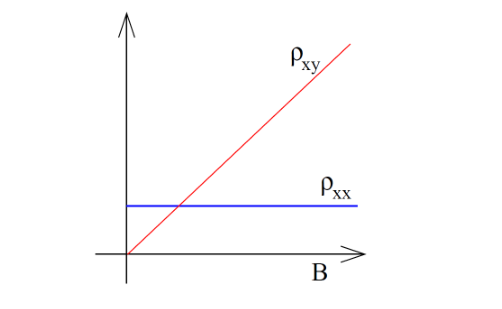
\includegraphics[width=8cm,height=4cm]{pic/1.png}
			\caption{经典霍尔效应横向纵向电阻率\cite{meng2018integer}}
		\end{center}
	\end{figure}
\end{frame}
\subsection{整数霍尔效应}
\begin{frame}{背景}
	\begin{figure}[H]
		\begin{center}
			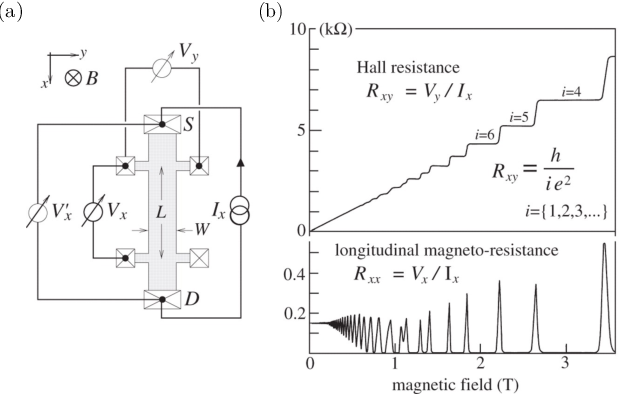
\includegraphics[width=8cm,height=4.4cm]{pic/2.png}
			\caption{$(a)$霍尔效应装置图$(b)R_{xx}$和$R_{xy}$随$B$大小变化图\cite{Abouzaid2018TheIQ}}
		\end{center}
	\end{figure}
\end{frame}
\begin{frame}{背景}
	\begin{center}
		{\Huge\calligra Why?}
	\end{center}
\end{frame}
\section{朗道能级}
\begin{frame}{朗道能级}
	\begin{block}{带电粒子在磁场下的运动}
		\begin{itemize}
			\item $\vec{B}=\nabla \times \vec{A}=B\hat{z}$
			\item $\hat{H}=\dfrac{1}{2m}(\hat{p}+e\hat{A})^{2}$
			\begin{itemize}
				\item $Landau\quad gauge:\vec{A}=xB\hat{y}(Why?)$
				\item $\hat{H}=\dfrac{1}{2m}(\hat{p_{x}}^{2}+(\hat{p_{y}}+eB\hat{x})^{2})$
			\end{itemize}
		\item $\psi_{k_{y}}=e^{ik_{y}y}f_{k_{y}}(x)$
		\item $\hat{H}\psi_{k_{y}}=(\dfrac{\hat{p_{x}}^{2}}{2m}+\dfrac{m\omega_{B}^{2}}{2}(\hat{x}+k_{y}l_{B}^{2})^{2})\psi_{k_{y}}$
		\begin{itemize}
			\item $\omega_{B}=\dfrac{eB}{m},\quad l_{B}=\sqrt{\dfrac{\hbar}{eB}}$
		\end{itemize}
	\item $E_{n}=(n+\dfrac{1}{2})\hbar\omega_{B}$
		\end{itemize}
	\end{block}
\end{frame}
\begin{frame}{朗道能级}
	\begin{block}{约束}
		\begin{itemize}
			\item 首先让我们把霍尔样品限制在一个有限的矩形区域$L_{x}\times L_{y}$。在$y$方向上我们有平面波,所以这等价于这个方向上盒子系统中的粒子。
			\item 动量量子化$k_{y}=\dfrac{2\pi N}{L_{y}}$
			\item 本征函数中心应该在样品内,逻辑约束:\\$x_{0}=-k_{y}l_{B}^{2}\le L_{x}\Rightarrow -L_{x}/l_{B}^{2}\le k_{y}\le 0$
			\item $N=\dfrac{L_{y}}{2\pi}\int_{-L_{x}/l_{B}^{2}}^{0}dk_{y}=\dfrac{eBL_{x}L_{y}}{2\pi \hbar}=\dfrac{\Phi}{\Phi_{0}}$
		\end{itemize}
	\end{block}
\end{frame}
\section{$SdH$振荡}
\subsection{边缘态}
\begin{frame}{$SdH$振荡}
\begin{itemize}
	\item 边缘态对于存在势能项的粒子而言不可忽略,因此我们用下图在临近边缘处突然上升的势场模拟边缘势场。
\end{itemize}
	\begin{figure}[H]
		\begin{center}
			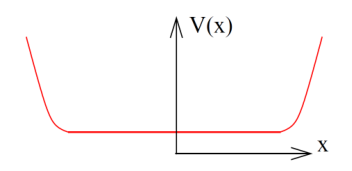
\includegraphics[width=8cm,height=4cm]{pic/3.png}
			\caption{样品势场分布\cite{meng2018integer}}
		\end{center}
	\end{figure}
\end{frame}
\begin{frame}{$SdH$振荡}
	\begin{block}{边缘态下的$Hamilton$量}
		\begin{itemize}
			\item{\small  $\begin{aligned}
				H_{k_{y}}&=\dfrac{p_{x}^{2}}{2m}+\dfrac{m\omega_{B}^{2}}{2}(k_{y}l_{B}^{2}+x)^{2}+x\dfrac{\partial V}{\partial x}\\
				&{\tiny =\dfrac{p_{x}^{2}}{2m}+\dfrac{m\omega_{B}^{2}}{2}((k_{y}l_{B}^{2}+\dfrac{\partial V}{\partial x}\dfrac{1}{m\omega_{B}^{2}})+x)^{2}-\dfrac{1}{2m\omega_{B}^{2}}(\dfrac{\partial V}{\partial x})^{2}-k_{y}l_{B}^{2}\dfrac{\partial V}{\partial x}}
			\end{aligned}$}
			\item $E_{n}=\hbar\omega_{B}(n+\frac{1}{2})-\frac{1}{2m\omega_{B}^{2}}(\frac{\partial V}{\partial x})^{2}-k_{y}l_{B}^{2}\frac{\partial V}{\partial x}$
			\item 群速度$v_{y}=\frac{1}{\hbar}\frac{\partial E}{\partial k_{y}}=-\frac{1}{eB}\frac{\partial V}{\partial x}$
			\item $I_{y}=-\frac{e}{L_{y}}\int dk_{y}\frac{L_{y}}{2\pi}v_{y}=\frac{e}{h}\Delta\mu$
			\item $V_{H}=\frac{\Delta \mu}{e}\Rightarrow \sigma_{xy}=\frac{I_{y}}{V_{H}}=\frac{e^{2}}{h}$
			\item 当我们将其扩展到多个朗道能级的填充的时候,可以得到:$\sigma_{xy}=\frac{ie^{2}}{h}$
		\end{itemize}
	\end{block}
\end{frame}
\subsection{霍尔电导量子化简单理解}
\begin{frame}{$SdH$振荡}
	\begin{block}{二维平面能量密度}
		\begin{itemize}
			\item 考虑无磁场二维电子气:$\kappa=\dfrac{2\pi}{L_{x}}\vec{i}+\dfrac{2\pi}{L_{y}}\vec{j},\quad E=\dfrac{\hbar \kappa^{2}}{2m}$
			\item 能量密度:$G(\kappa)d\kappa=\dfrac{2\pi\kappa d\kappa}{2\pi/L_{x}\times2\pi/L_{y}}$
			\item 单位面积态密度:$g(E)=\dfrac{G(E)}{L_{x}L_{y}}=\dfrac{m}{2\pi\hbar^{2}}$
		\end{itemize}
	\end{block}

\end{frame}
\begin{frame}{$SdH$振荡}
\begin{block}{霍尔电导量子化}
	\begin{itemize}
		\item 电子朗道能级差为:$\hbar\omega_{B}$,能级简并度为:$g(E)\times \hbar\omega_{B}=\dfrac{Be}{h}$
		\begin{itemize}
			\item 电子只能处于分立的能级,每个能级的电子数为$\dfrac{Be}{h}$
		\end{itemize}
		\item 假设电子填满了$i$个能级,$N=i\times \dfrac{Be}{h}$,\quad$\sigma_{xy}=\dfrac{Ne}{B}=\dfrac{ie^{2}}{h}$
	\end{itemize}
\end{block}	
\end{frame}

\begin{frame}{$SdH$振荡}
	\begin{block}{$TKNN$方程}
\begin{figure}[H]
	\centering
	\subfigure{
		\begin{minipage}[t]{0.3\linewidth}
			\centering
			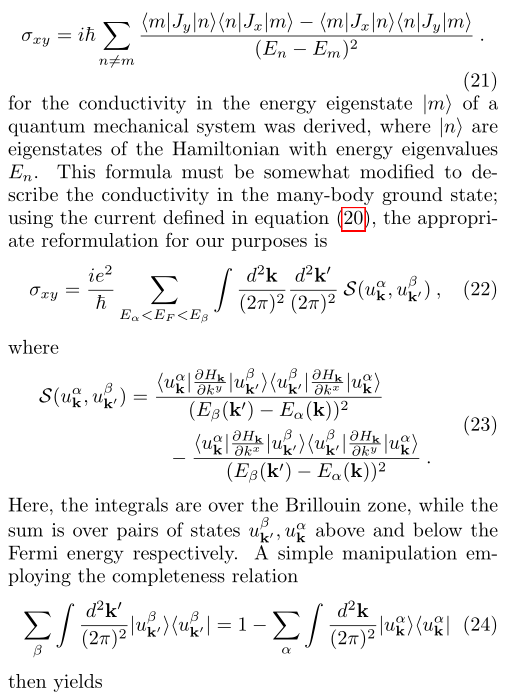
\includegraphics[width=1.2in]{pic/4.png}
			%\caption{fig1}
		\end{minipage}%
	}%
	\subfigure{
		\begin{minipage}[t]{0.3\linewidth}
			\centering
			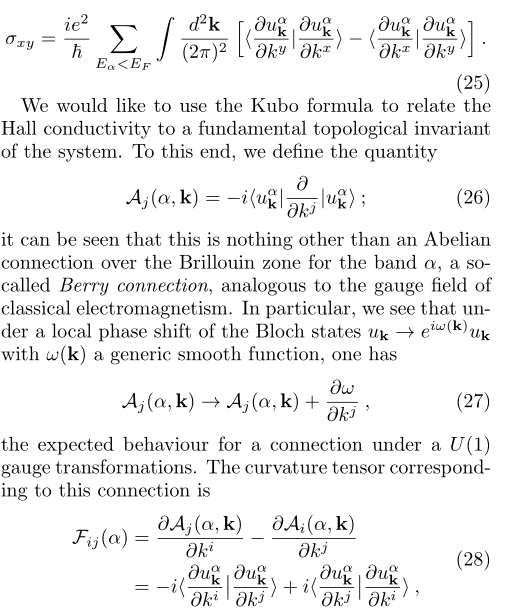
\includegraphics[width=1.4in]{pic/6.png}
			%\caption{fig2}
		\end{minipage}%
	}%
	\subfigure{
		\begin{minipage}[t]{0.3\linewidth}
			\centering
			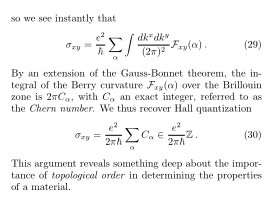
\includegraphics[width=1.7in]{pic/5.png}
			%\caption{fig2}
		\end{minipage}
	}%
	\centering
\end{figure}
	\end{block}
\end{frame}
\subsection{样品中的缺陷}
\begin{frame}{$SdH$振荡}
	\begin{itemize}
		\item 稳定情况($\tau \rightarrow \infty$):$\rho_{xx}=0,\rho_{xy}=\dfrac{B}{ne}$
		\item 为什么$\rho_{xx}$会出现振荡形式?
	\end{itemize}
\begin{block}{$SdH$振荡物理机制}
	在每个朗道能级中,电子状态数($\frac{Be}{h}$)随磁场的增加而线性增加。因此,随着磁场的增大,朗道能级会向能量更高的方向移动。当每一个能级通过费米面时,电导就会减小随着能带里面的电子变为自由电子流动起来,这导致材料的电导率呈周期性地振荡。
\end{block}
\end{frame}
\begin{frame}{$SdH$振荡}
	\begin{figure}[H]
	\begin{center}
		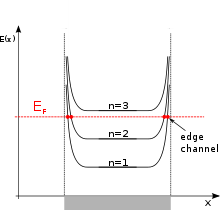
\includegraphics[width=4.5cm,height=2.5cm]{pic/9.png}
		\begin{itemize}
			\item 费米面$E_{F}$位于两个朗道能级之间。当能带穿过费米面$E_{F}$时,它们中的电子就会变得可移动。由于费米面$E_{F}$位于两个朗道能级之间,电子的散射只发生在向上弯曲的样品边缘($Why?$),相对应的电子态通常被称为边缘通道。
			\item $Landauer$公式:$G=\dfrac{2e^{2}}{h}T$($Why?$)
			\item $Buttiker$公式:$I_{p}=\sum\limits_{q}G_{pq}(V_{p}-V_{q})$
			\begin{itemize}
				\item 其中$I_{p}$为$p$端口的电流,$G_{pq}$为从端口$q$到端口$p$的电导,$V_{p},V_{q}$为$p,q$的电压
			\end{itemize}
		\end{itemize}
	\end{center}
\end{figure}
\end{frame}
\begin{frame}{$SdH$振荡}
	\begin{block}{六端口通道($T=2$)}
			\begin{figure}[H]
			\begin{center}
				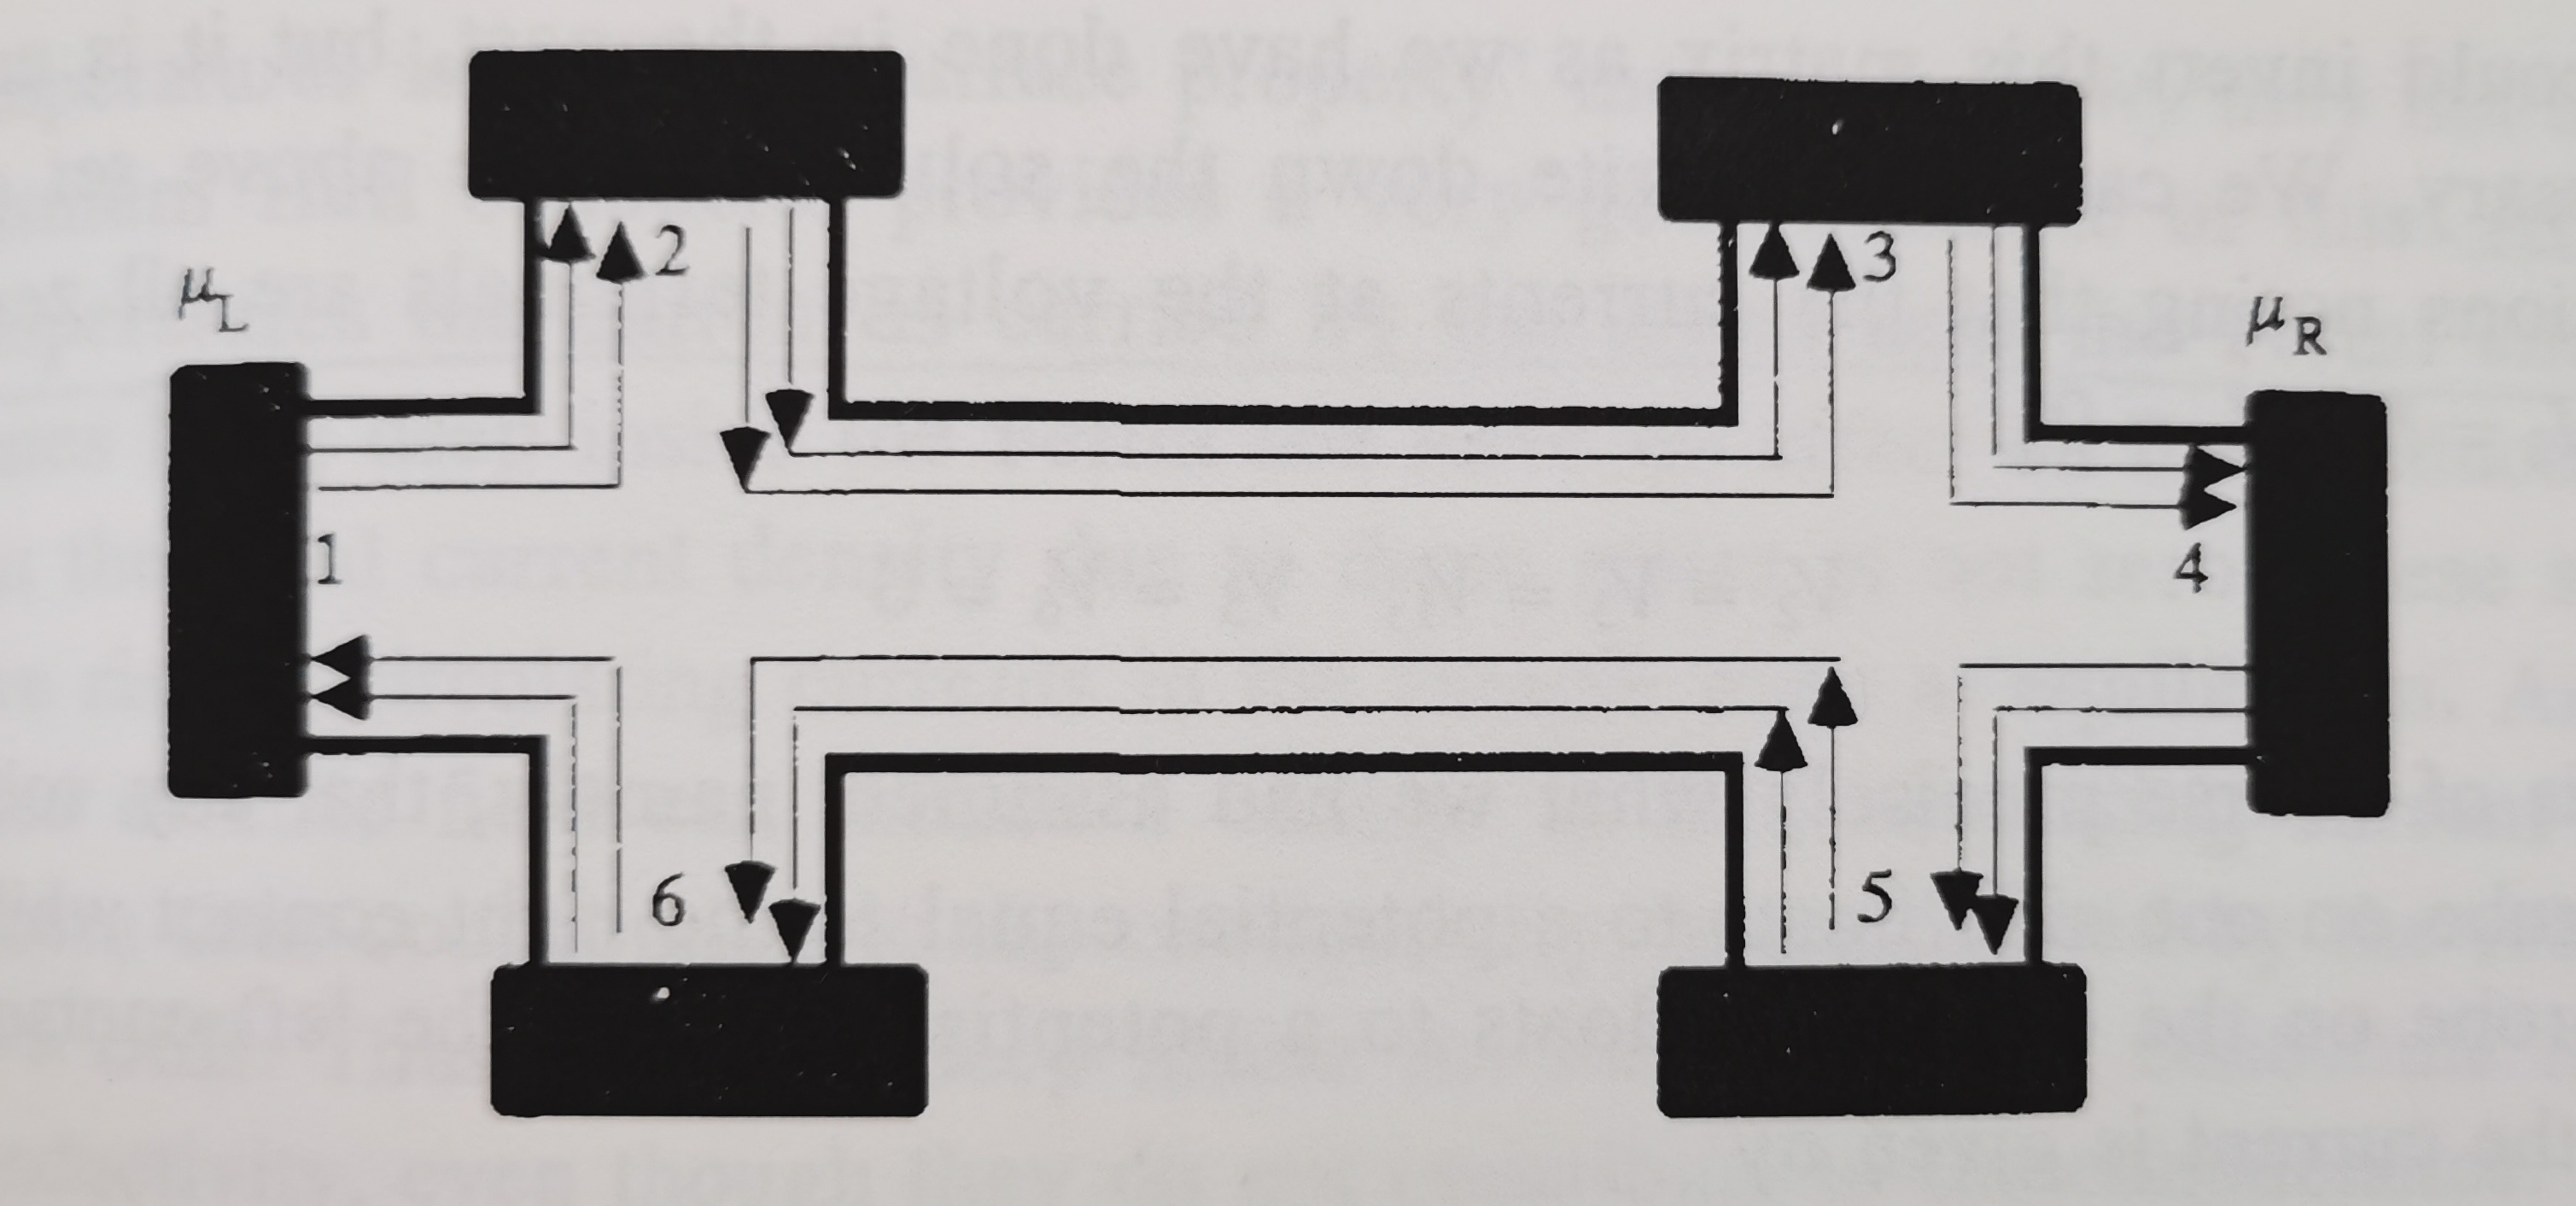
\includegraphics[width=5.5cm,height=2.5cm]{pic/10.jpg}
			\end{center}
		\end{figure}
	\begin{itemize}
		\item $\begin{pmatrix}
			I_{1}\\
			I_{2}\\
			I_{3}\\
			I_{4}\\
			I_{5}\\
			I_{6}\\
		\end{pmatrix}$=$\begin{pmatrix}
		G_{c}&0&0&0&0&-G_{c}\\
		-G_{c}&G_{c}&0&0&0&0\\
		0&-G_{c}&G_{c}&0&0&0\\
		0&0&-G_{c}&G_{c}&0&0\\
		0&0&0&-G_{c}&G_{c}&0\\
		0&0&0&0&-G_{c}&G_{c}\\
	\end{pmatrix}$$\begin{pmatrix}
	V_{1}\\
	V_{2}\\
	V_{3}\\
	V_{4}\\
	V_{5}\\
	V_{6}\\
\end{pmatrix}$
	\end{itemize}
	\end{block}
\end{frame}
\begin{frame}{$SdH$振荡}
	\begin{itemize}
		\item $I_{2}=I_{3}=I_{5}=I_{6}=0$
		\item $R_{x}=\dfrac{V_{2}-V_{3}}{I}=\dfrac{V_{6}-V_{5}}{I}=0$
		\item $R_{H}=\dfrac{V_{2}-V_{6}}{I}=\dfrac{V_{3}-V_{5}}{I}=G_{c}^{-1}=\dfrac{h}{2e^{2}}$
	\end{itemize}
\end{frame}
\begin{frame}{$SdH$振荡}
	\begin{block}{引入杂质}
		\begin{itemize}
			\item 我们使用一个在朗道能级附近的随机势模拟杂质的影响
			\begin{figure}[H]
				\begin{center}
					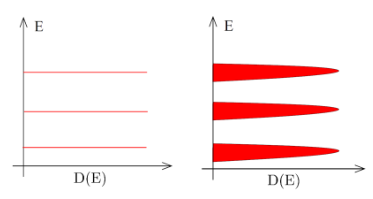
\includegraphics[width=8cm,height=4cm]{pic/7.png}
					\caption{纯净样品与有杂质样品的能态分布\cite{meng2018integer}}
				\end{center}
			\end{figure}
		\end{itemize}
	\end{block}
\end{frame}
\begin{frame}{$SdH$振荡}
		\begin{figure}[H]
		\begin{center}
			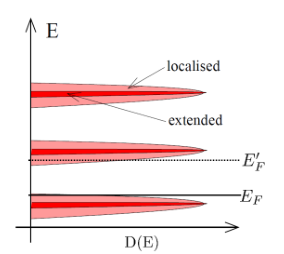
\includegraphics[width=4.5cm,height=3cm]{pic/8.png}
		\end{center}
	\end{figure}
	\begin{figure}[H]
	\begin{center}
		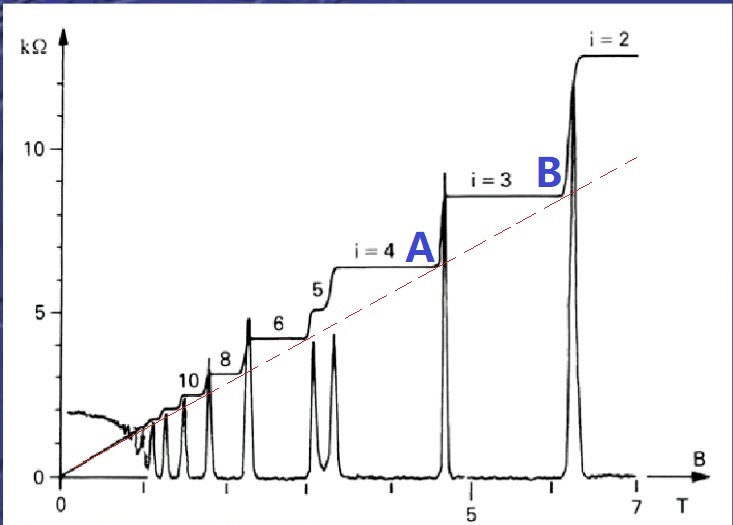
\includegraphics[width=5cm,height=2.6cm]{pic/4.jpg}
	\end{center}
\end{figure}
\end{frame}
\begin{frame}{$SdH$振荡}
	\begin{block}{为何$R_{xy}$会有平台或者突变出现}
		\begin{itemize}
			\small 
			\item 假设此时磁场加在$A$的位置,这时电子占满了四个能级,总的电子面密度和不考虑量子效应时相等($A$点也在红色虚线上),这时加大磁场,能级简并增大,总电子数占满了前三个能级后,占不满第四个能级,这些“多余”的电子被挤向了“局域态”,它是由缺陷导致的,好像电子被束缚在原子核周围,这些电子不参与导电,这样参与导电的电子突然减少,就会导致图中霍尔电阻的徒然上升
			\item 杂质使得朗道能级展宽,但是杂质态是局域的,局域态不导电,因此费米能级在展宽的朗道能级内移动时,电导不发生改变,行程电导平台,平台的宽度和杂质态展宽的朗道能级宽度有关
			
		\end{itemize}
	\end{block}
	
\end{frame}
\begin{frame}{$SdH$振荡}
	\begin{block}{为何$R_{xx}$会变为0}
		\begin{itemize}
			\item 因为基态和激发态之间存在能隙,在极低温度下,电子既不能获得足够能量跃迁,又不能前往已经占满的低能态,无处可去的电子只能挤在一起,形成所谓的超流,不会受到散射,故不需要额外的电场驱动就能维持电流,类似于光滑平面的匀速运动,所以水平电阻$R_{xx}=0$
			\item 当磁场继续增大至图中$B$点,局域态中的电子已经完全进入前三个能级上,此时的霍尔电阻又和经典情况一样,继续增加磁场,超流态破坏,部分电子又变成局域态,会有强烈散射,水平方向的电阻又不为0,出现一个峰值
		\end{itemize}
		
	\end{block}
\end{frame}
\begin{frame}{$SdH$振荡}
	\begin{center}
		{\huge\calligra Question:}\\
		量子霍尔效应中平台在朗道能级吗?
	\end{center}
\end{frame}
\begin{frame}{$SdH$振荡}
	\begin{center}
		{\huge\calligra Question:}\\
		量子霍尔效应杂质越少越好吗?
	\end{center}
\end{frame}
\section{参考文献}
\begin{frame}{参考文献}
	\printbibliography[heading = bibintoc]
\end{frame}
\begin{frame}
    \begin{center}
        {\Huge\calligra Thanks!}
    \end{center}
\end{frame}

\end{document}
